%*****************************************
\chapter{Theory and Alternatives}\label{ch:theory_and_alternatives}
%*****************************************


\section{Means-End Analysis}

In 1959, Newell, Shaw, and Simon published a report on a means-end
analysis model that was designed to solve any symbolically represented
problem \citep{newell:1959}.  Their system was called the \ac{GPS},
and worked by being able to work with relational representations of
current and desired states.  The agent had a catalogue of differences
between states that it knew how to minimize.  The system worked by
finding the largest difference and executing the associated method for
reducing this difference.  This work has grown into the Soar model
\citep{newell:1990} for better solving symbolic planning problems, and
dealing with impasses for when the planning search runs out of
options.

\section{Difference-Engine Model for Accomplishing Multiple Goals}

\begin{figure}[bth]
  \center
  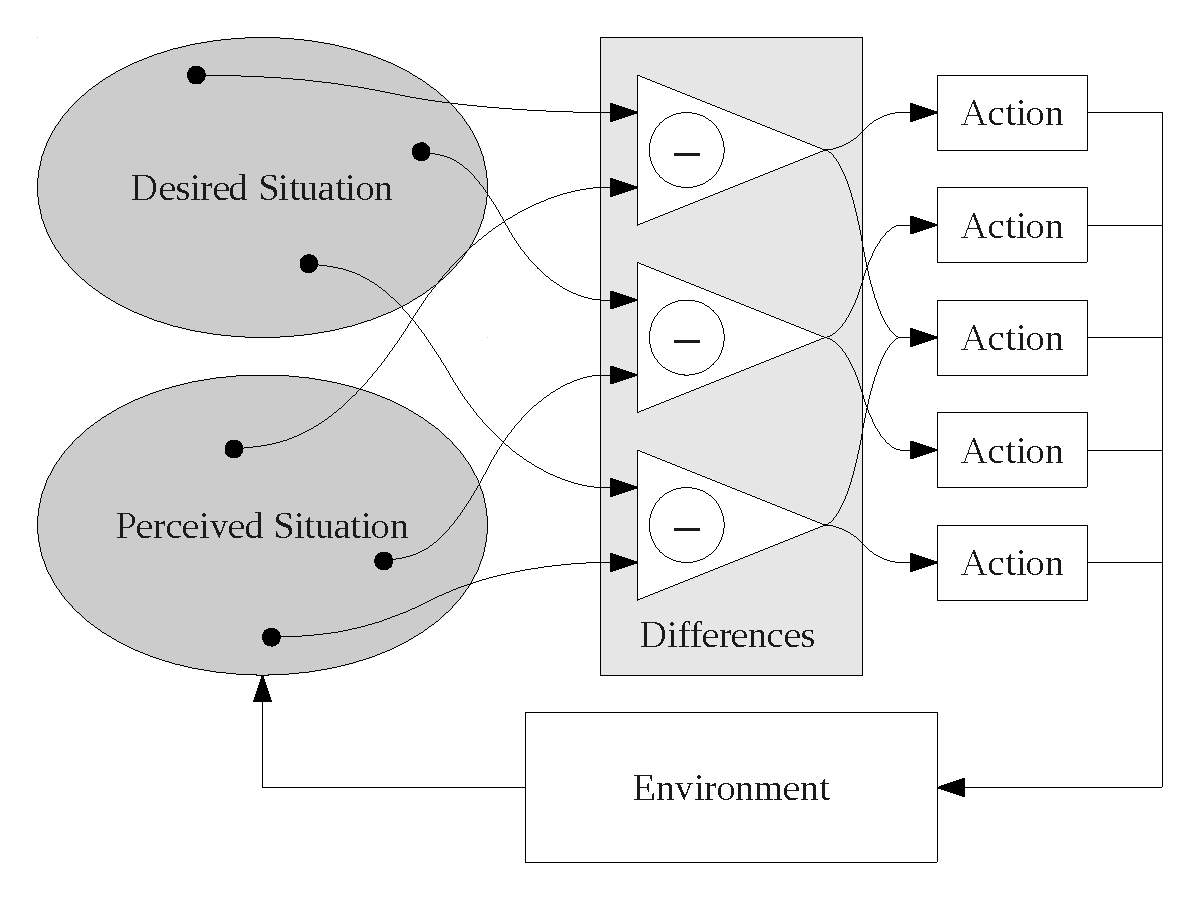
\includegraphics[height=6cm]{gfx/difference_engine_feedback_control}
  \caption[The difference engine model for accomplishing multiple goals]{The difference engine model for accomplishing multiple goals.}
  \label{fig:difference_engine_feedback_control}
\end{figure}

\citep[p.~78]{minsky:1988}


